
\section{Overview}

In this chapter, we present the results of our analysis. This consists of the invariant cross section for $\pi^0$ and $\eta$ mesons using Run 24 \ac{pp} data, both as functions of $p_T$ and pseudorapidity ($\eta$). The invariant cross section, along with the $\eta$ to $\pi^0$ ratio, was compared with previous \ac{PHENIX} measurements wherever applicable. As discussed in previous chapters, the results were obtained using a combination of minimum bias and two types of photon-triggered data sets.


\section{Invariant Mass Peak and Width}

The first measurement was the mass (signal peak) for both $\pi^0$ and $\eta$ mesons. We measured peak positions as a function of transverse momentum ($p_T$) to verify the consistency of mass (peak mean) and sigma (width). To calculate this, we constructed an invariant mass histogram using golden parameter cuts. Then, using a side-band fitting process, estimate complete background and subtracted it to get a signal distribution. The final step we did was to fit the signal distribution using a Gaussian function to extract the mean and sigma of the meson peak. The range of fitting gaussian function was $0.06 \le m_{\gamma \gamma} \le 0.25$ for $\pi^0$ and $0.38 \le m_{\gamma \gamma} \le 0.76$ for $\eta$ mesons.

The figure \ref{fig:pi0_mass_sigma} suggest that the mass and sigma distributions are consistent as a function of $p_T$ and across all three triggered data. In Figure \ref{fig:pi0_mass_sigma}, we can see sharp rise in mass and sigma for $p_T \geq 6 $ \ac{GeV}. This effect is due to merging behavior of $\pi^0$ photons, which limits our $\pi^0$ analysis at very high $p_T$.

Similarly, $\eta$ mesons show a small and gradual drop in both mass and sigma on increasing $p_T$. This is caused by our method of signal extraction and a better $S/B$ ratio in the higher $p_T$ range. However, this difference is insignificant (just a few percent), so we can assume constant behavior of mass and sigma for the $\eta$ meson as well.


\begin{figure}[H]
%\begin{figure}[tbh]
    \centering

    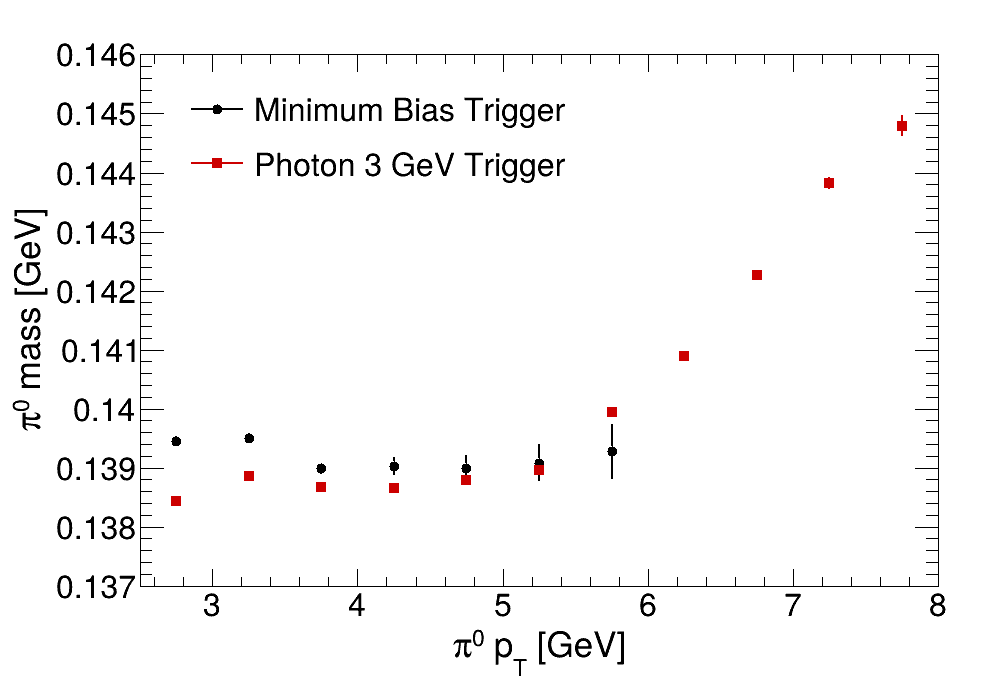
\includegraphics[width=0.9\textwidth,
      alt={Plot of the neutral-pion mass versus transverse momentum from 2.75
           to 7.75 GeV for the minimum-bias trigger (black) and the Photon
           3 GeV trigger (red). The mass stays near 0.139 GeV up to about
           5.5 GeV and then rises to about 0.145 GeV.}]{Images/6_Plots/pi0_peak_vs_pT.png}

    \vspace{0.5cm} % Adjust vertical spacing if needed

    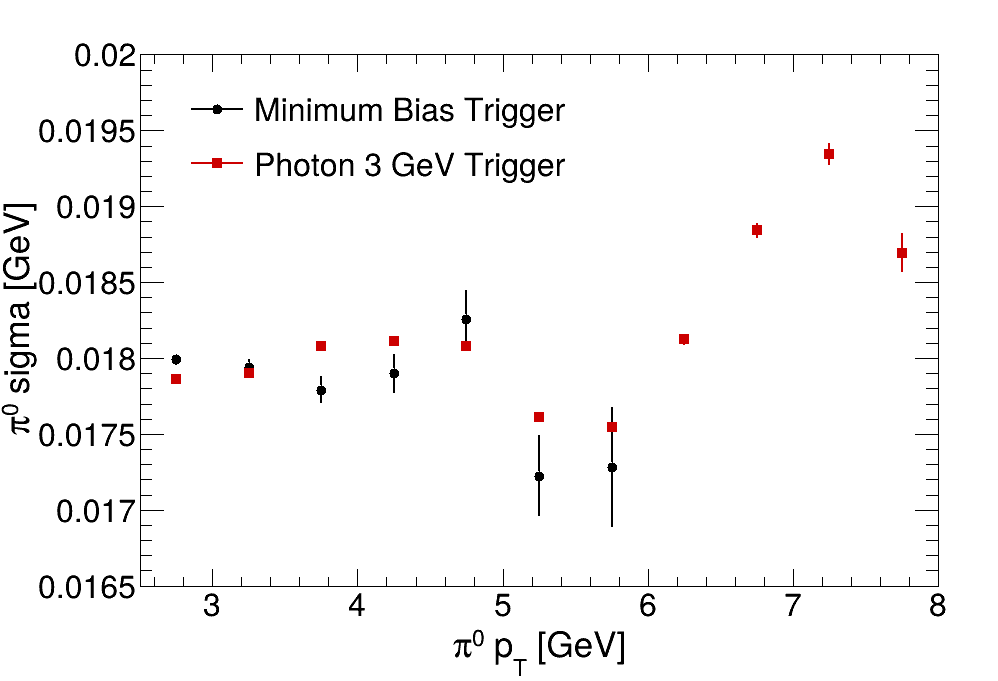
\includegraphics[width=0.9\textwidth,
      alt={Plot of the neutral-pion peak width (sigma) versus transverse
           momentum from 2.75 to 7.75 GeV for the minimum-bias trigger (black)
           and the Photon 3 GeV trigger (red). The width is about 0.018 GeV at
           low momentum and increases to about 0.019 GeV above
           6 GeV.}]{Images/6_Plots/pi0_sigma_vs_pT.png}

    \caption{Distribution of $\pi^0$ mass (\textbf{top panel}) and sigma (\textbf{bottom panel}) as a function of transverse momentum ($p_T$). The error in both plots are obtained from the fitting procedure.}
    
    \label{fig:pi0_mass_sigma}
  
\end{figure}


